\chapter*{Medlemskortprosjektet}
\addcontentsline{toc}{chapter}{Medlemskortprosjektet}

Vedtak fra Finansstyertes referater:


\begin{instruksledd}{SAK 22/02 Medlemskortprosjektet}
    Andreas Jordell og Amund Tøftum redegjorde for status for medlemskortprosjektet.
    ``Markedsplan medlemskort
    Studentersamfundet'' ble overlevert. Rapporten er skrevet i forbindelse med faget
    ``Markedsføring og entreprenørskap''
    ved NTNU.
    
    \textbf{Vedtak:}

    Finansstyret gir sin tilslutning til medlemskortprosjektets framlagte visjon og
    målsetninger. Finansstyret ber om at
    budsjett for kam

\end{instruksledd}

\begin{instruksledd}{SAK 19/03 Medlemskortprosjektet}
    Medlemskortprosjektet ble satt i gang våren 2002 for å bidra til å øke medlemstallet
    ved Studentersamfundet. Andreas
    Jordell går av etter et år som leder for prosjektet og det skal settes sammen en ny
    gruppe.
    
    Gjengsekretariatet har innstilt Christian Waale Hansen som ny leder for perioden fram
    til våren 2004.
    
    \textbf{Vedtak:}

    Finansstyret takker Andreas Jordell for god innsats i jobben som leder for
    Medlemskortprosjektet 2002/2003.
    Finansstyret godkjenner Christian Waale Hansen som ny leder for Medlemskort-prosjektet
    og ønsker lykke til i
    oppfølgingen og videreføringen av Medlemskortprosjektet 2002/2003.
    
    Finansstyret ber Gjengsekretariatet følge opp videre arbeid i Medlemskortprosjektet og
    koordinere budsjettering av
    høstens tiltak. Finansstyret anser at det er satt av tilstrekkelige midler til tiltak
    i driftsbudsjettet.


\end{instruksledd}


\begin{instruksledd}{SAK 18/05 Sluttrapport fra Medlemskortprosjektet}
    Medlemskortprosjektet ble opprettet i 2002 med formål å øke salget av medlemskort,
    samt se på utviklingen av dette.

    Prosjektet går nå mot slutten og prosjektleder Christian Waale Hansen har levert en
    sluttrapport til Finansstyret.
    
    \textbf{Vedtak:}

    Finansstyret tar Medlemskortprosjektets rapport til orientering og berømmer gruppen
    for innsatsen.
    
    Det bes om at Medlemskortprosjektet leverer en innstilling til Finansstyret på møtet i
    august, hvor ansvarsplassering
    for videre oppfølging klargjøres.
\end{instruksledd}


\chapter*{Nybygg på Fengselstomta}
\addcontentsline{toc}{chapter}{Nybygg på Fengselstomta}

Vedtak gjort i Finansstyrets møter som omhandler arbeidet med Klostergata 9,
``Fengselstomta'':

\begin{instruksledd}{SAK 16/03 Videre arbeid med Fengselstomta}
    
    \textbf{Vedtak:}
    
    Finansstyret ønsker å vurdere alternativer for utbygging av Fengselstomta, Klostergata
    9.

    Finansstyret nedsetter en arbeidsgruppe bestående av Gisle Aasgaard, Hans Bøhle Aarhus
    og Håvard Hamnaberg
    (leder) som bes utrede muligheter og skissere en eventuell løsning, inklusive
    arealbehov, byggemulighet, finansiering,
    eierskap og prosjektorganisering.
    
    20. mai 2003

\end{instruksledd}

\begin{instruksledd}{SAK 26/03 Fengselstomta}
    Arbeidsgruppa som ble nedsatt i mai (sak 16/03) har levert rapport og skisse til
    videre arbeid. Håvard Hamnaberg
    redegjorde på møtet. Det planlegges nå med en bygning i størrelsesorden 1000 m². NTNU
    har gitt tilsagn om
    7 millioner til prosjektet. En viktig del av det videre arbeidet er å sikre øvrig
    finansiering til prosjektet.

    \textbf{Vedtak:}
    
    Finansstyret går inn for å fortsette arbeidet med løsningen som er foreslått av
    arbeidsgruppen som ble opprettet i mai,
    se sak 16/03. Finansstyret ber arbeidsgruppen fortsette utredningen og rekruttere
    medlemmer etter behov.
    
    Finansstyret vedtar å fremme følgende sak for Studentersamfundet:
    «Studentersamfundet i Trondhjem, samlet til møte 17. september 2003, ber Finansstyret
    arbeide videre med planene
    om å realisere et bygg på eiendommen Klostergata 9, ’Fengselstomta’, innen rammene som
    er presentert.»
    
    2. september 2003

\end{instruksledd}

\begin{instruksledd}{SAK 08/04 Fengselstomta}
    Prosjektgruppen som har arbeidet med utbygging av Fengselstomta har i samarbeid kommet
    fram til et løsningsforslag
    der NTNU setter opp et bygg som Studentersamfundet kan benytte vederlagsfritt. NTNU
    vil eie bygg og tomt, mens
    Studentersamfundet vil står for driften av bygget. Ved videre utbygging av eiendommen
    vil Studersamfundet ha
    mulighet til å øke arealet ytterligere.
    
    Foreløpige kalkyler viser at Studentersamfundet må regne med følgende engangskostnader
    ved en utbygging: Inventar
    med 500.000 kroner og tilpasninger av Samfundsbygningen med 750.000 kroner. Videre
    regnes det med at årlige
    driftskostnader i intervallet 400.000 – 600.000 kroner for bygningen, noe som
    tilsvarer 40-80\% av resultatet fra
    kafèdriften utenom helgene. Videre peker man på at deler av arealet er tiltenkt
    enheter med egen økonomi og at disse
    kan dekke deler av driftskostnadene.
    Det er ønskelig å behandle saken i Studentersamfundet før videre avtalearbeid og
    forprosjektering – noe som kan
    gjøres sommeren 2004. Styret har foreslått å avholde Samfundsmøte 19. mai 2004.
    
    \textbf{Vedtak:}

    Finansstyret går inn for å fortsette arbeidet med framlagt løsning for realisering av
    et bygg på eiendommen
    Klostergata 9 i samarbeid med NTNU.
    
    Finansstyret vedtar å fremme følgende sak for Studentersamfundet:.
    
    \begin{quote}
        Studentersamfundet i Trondhjem, samlet til møte 19. mai 2004, gir sin tilslutning til
        framlagte planer og
        løsningsrammer for å realisere et bygg på eiendommen Klostergata 9, ``Fengselstomta''.
        Finansstyret gis fullmakt til å inngå avtaler med NTNU om bebygging og bruk av
        eiendommen, herunder fullmakt til å
        overdra eiendommen Klostergata 9 til NTNU.
    \end{quote}

    Finansstyret ber Styret avholde Samfundsmøte der saken kan behandles, fortrinnsvis 19.
    mai 2004.

    11. mai 2004

\end{instruksledd}

\begin{instruksledd}{SAK 22/04 Fengselstomta – romplan og organisering fremover}
    Fengselstomtprosjektet (FTP) har utarbeidet en romplan for nybygg på fengselstomta.
    FTP har i romplanen lagt vekt
    på å avlaste offentlige arealer, bedre arbeidsforholdene for ansatte, bedre
    arbeidsforholdene for Mediastud og
    festivalene samt frigjøre private arealer. Romplanen har vært til høring hos alle
    gjengene.

    FTP ønsker i sitt videre arbeid å fortsette med Håvard Hamnaberg som leder, Hallstein
    Havåg og Eirik Sæther, samt
    knytte til seg nye medlemmer for videre arbeid med byggeprosjektet på Fengselstomta og
    konsekvenser dette vil få i
    Samfundsbygningen.
    
    \textbf{Vedtak:}

    Finansstyret gir tilslutning til fremlagte forslag til romplan for nybygg på
    fengselstomta. FTP gis fullmakt til å gjøre
    mindre vesentlige endringer i romplanen.
    
    Finansstyret ber eksisterende arbeidsgruppe arbeide videre med realiseringen av
    fengselstomtprosjektet med
    Hamnaberg som leder. Gruppen gis fullmakt til å rekruttere nye medarbeidere, slik at
    gruppen vil utgjøre 10
    medlemmer totalt.
    
    Finansstyret forventer kontinuerlig rapportering.
    
    5. oktober 2004

\end{instruksledd}


\begin{instruksledd}{SAK 29/04 Utbygging av Klostergata 9 (Fengselstomta)}
    Fengselstomtprosjektet v/leder Håvard Hamnaberg orienterte om status for prosjektet:
    Rekrutteringen er ferdig og
    prosjektorganisasjonen er fulltallig. Prosjekteringsarbeidet rundt nybygget er stilt i
    bero i påvente av løsning for veien
    bak Samfundsygningen; det ventes en avklaring i mai 2005.

    Det pågår forhandlinger med NTNU om avtaleverket for eiendomsoverdragelsen og
    utbyggingen. Hamnaberg
    presenterte struktur og prinsipper for avtaleverket.
    
    Det er gjort en initiell analyse av kostnadene som må bæres av Studentersamfundet. Det
    kan regnes med 200 tusen
    kroner til prosjektering av ombygginger i Samfundsbygningen i 2005, mens kostnader til
    ombyggingen anslås til 2
    millioner kroner, der 50\% søkes dekket av eksterne bidragsytere, og inngår i revidert
    vedlikeholdsplan for perioden
    1997-2006. Det kan videre regnes med 300 tusen kroner til anskaffelse av inventar i
    2006.

    \textbf{Vedtak:}

    Finansstyret er tilfreds med resultatene fra arbeidet i Fengselstomtprosjektet så
    langt. Finansstyret ber
    Fengselstomtprosjektet innhente en tredjepartsvurdering av avtaleverket med hensyn på
    ivaretakelse av
    Studentersamfundets langsiktige interesser i eiendommen og bygningen.
    
    16. november 2004


\end{instruksledd}


\begin{instruksledd}{SAK 09/05 Fengselstomtutbygging}
    Forhandlingene med NTNU har ført fram til forslag til avtaler: Intensjonsavtale for
    utbyggingen, avtale om salg av
    eiendommen og langsiktig leieavtale for bygget. Prinsippene i avtalene er at NTNU vil
    sette opp et bygg etter
    Studentersamfundes ønsker og retningslinjer på rundt 1000 kvm, innenfor en ramme på 22
    millioner kroner.
    Studentersamfundet vil leie bygningen vederlagsfritt i 99 år og stå for driftsutgifter
    og indre vedlikehold. NTNU vil
    overta eiendommen Klostergata 9 gratis og kunne disponere denne til videre utbygging.
    Inntil videre utbygging vil
    bruk av av tomten kunne avtales med NTNU, mens ved en utbygging vil Studentersamfundet
    ha mulighet til å
    forhandle om mer arealer.

    På den tekniske siden er det tegnet et skisseprosjekt og utarbeidet en romplan.
    Prosjekteringsarbeidet rundt nybygget
    er stilt i bero i påvente av løsning for veien bak Samfundsbygningen. Det er satt
    igang en reguleringsprosess som
    normalt tar ett år regnet fra sommeren 2004. Videre arbeides det med å justere
    eiendomsgrensene mellom
    Fengselstomta og Samfundsbygningen. Tidsaspektet for disse prosessene fører til at
    utbyggingen må legges fram til
    behandling i Studentersamfundet.

    \textbf{Vedtak:}

    Finansstyret gir sin tilslutning til framlagte forslag til avtaler om salg, utbygging
    og bruk av eiendommen Klostergata
    9, Fengselstomta.

    Finansstyret vedtar å fremme følgende sak for Studentersamfundet: 
    \begin{quote}
        Studentersamfundet i Trondhjem, samlet til møte
        20. april 2005, gir sin tilslutning til prinsippene i framlagte avtaler og planer for
        å realisere et bygg på eiendommen
        Klostergata 9, ``Fengselstomta'', herunder overdragelse av eiendommen Klostergata 9 til
        NTNU og inngåelse av en
        langsiktig leieavtale i et bygg reist av NTNU. Finansstyret gis fullmakt til å inngå
        avtaler med NTNU om utbygging,
        salg, leie og bruk av eiendommen. Fullmakten omfatter redaksjonelle endringer av
        avtalene innenfor framlagt
        prinsipper og gis en varighet på et år.
    \end{quote}

    Forutsatt tilslutning fra Studentersamfundet gir Finansstyret leder fullmakt til å
    inngå avtaler på vegne av Finansstyret
    vedrørende salg, utbygging og leie av Klostergata 9, herunder å signere dokumenter
    sammen med Studentersamfundets leder.
    
    5. april 2005

\end{instruksledd}


\begin{instruksledd}{SAK 23/05 Oppnevning av ny leder for Fengselstomtprosjektet}
    I sak 16/03 ble Fengselstomtprosjektet (FTP) opprettet med Håvard Hamnaberg som leder,
    for å utrede muligheter for
    nybygg på fengselstomta. Hamnaberg har nå gitt beskjed om at han ønsker å fratre som
    leder i FTP.

    \textbf{Vedtak:}

    Finansstyret utnevner Hallstein Havåg som ny leder av Fengselstomtprosjektet.
    
    24. mai 2005
\end{instruksledd}

\begin{instruksledd}{SAK 24/05 Konsekvensprosjektet – ansvar for oppfølging}
    I forbindelse med den planlagte utbyggingen på Fengselstomta vil en del av de
    offentlige og private arealene i dagens
    Samfundsbygning måtte omdisponeres og/eller ombygges. Dette er en nødvendig del av
    arbeidet med å maksimere
    effekten av nybygget slik at det kommer flest mulig av Samfundets ansatte og aktive
    til gode. En plan for disse
    omdisponeringene må gjøres samlet for å få en helhetlig løsning, og må være klar i god
    tid før nybygget står ferdig.

    \textbf{Vedtak:}

    Finansstyret ber Fengselstomtprosjektet lede prosessen med ombygginger av
    Samfundsbygningen som konsekvens av
    utbyggingen på fengselstomta. Det er en forutsetning at arbeidet blir gjennomført i
    forståelse med gjengene på Huset, D-gjengen og Samfundets byggekomit.
\end{instruksledd}
\pagebreak






%ugly ugly UGLY UGLY UGLY bugly!!
\begin{center}
	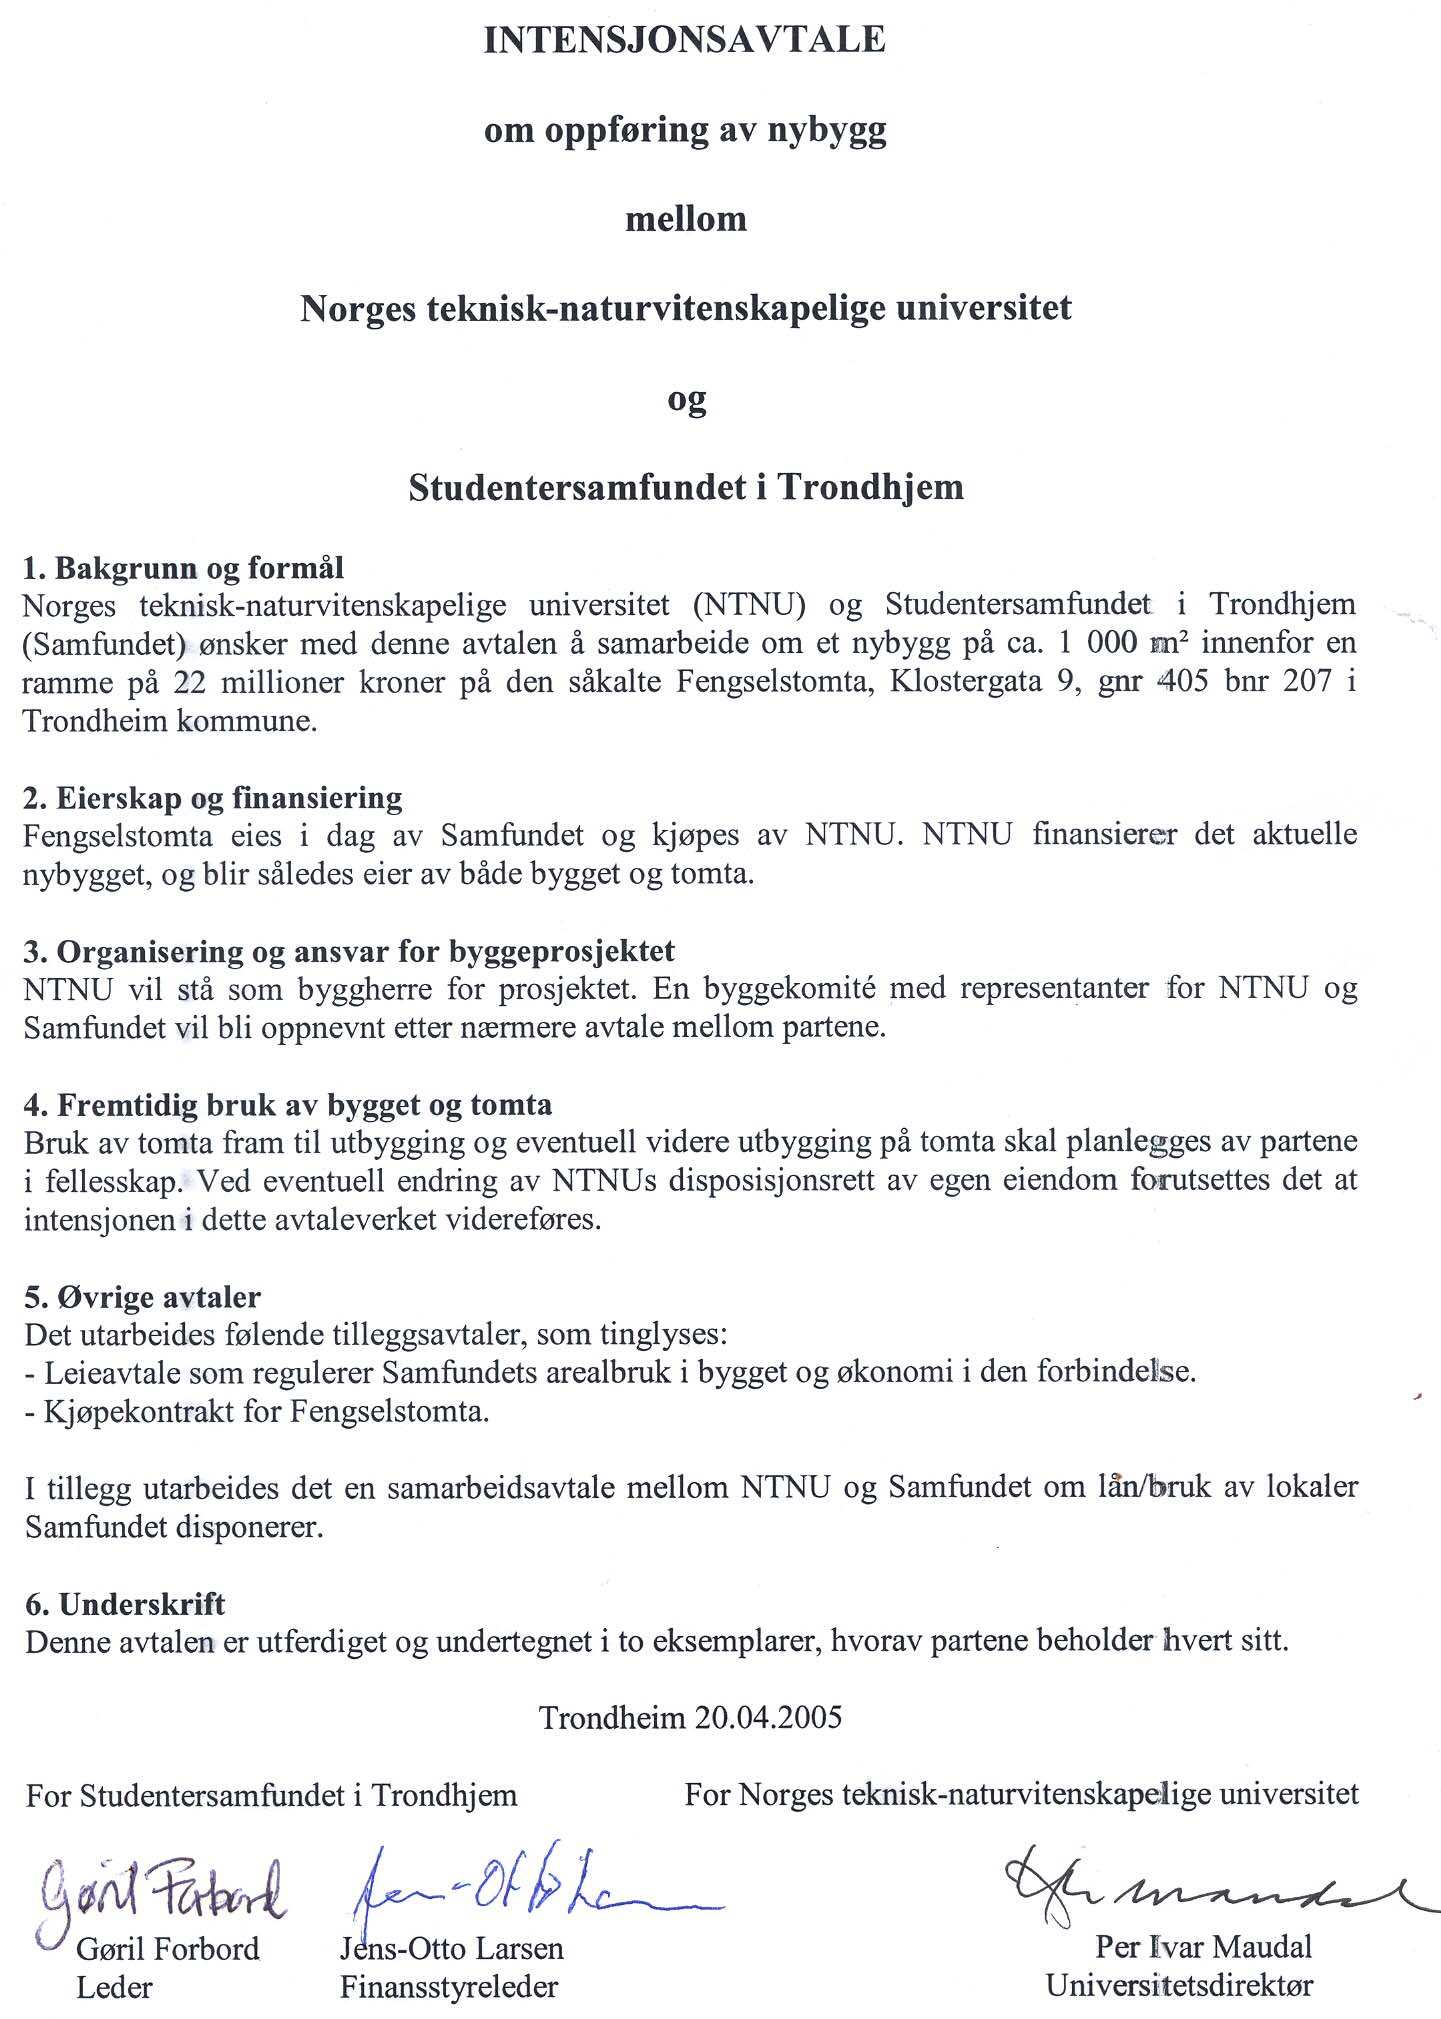
\includegraphics[width=\textwidth]{AvtaleOmNybygg}
\end{center}



